\documentclass{article}

\usepackage[a4paper, total={6in, 8in}]{geometry}
\usepackage[utf8]{inputenc}
\usepackage{fancyhdr}
\usepackage{graphicx}
\usepackage{enumitem}

\pagestyle{fancy}
\fancyhf{}
\lhead{John J Li}
\rhead{CSE360 Summer 2021 Notes}
\rfoot{\thepage}
\renewcommand{\headrulewidth}{0.4pt}

\setlength{\parskip}{1em}
\setlength\parindent{0px}
\title{CSE360 Summer 2021 Notes}
\date{\today}
\author{John J Li}

\begin{document}
    \section*{Information Management}

    Information Management System (IMS)
    \begin{itemize}
        \item General term for software systems designed to facilitate the storage, organization, and retrieval of information
        \item Sometimes used synonymously with Database Management System (DBMS)
        \item Data is stored in a variety of formats
        \item Makes it easier to access stored information
    \end{itemize}

    Steps when designing a database
    \begin{itemize}
        \item Requirements collection and analysis
        \item Conceptual design
        \item Choose a DBMS
        \item Logical Design
        \item Physical Design
        \item Implementation
    \end{itemize}

    \subsection*{IMS/DBSMS vs RDBMS}

    Information Management System (IMS)
    
    Database Management System (DBMS)
    \begin{itemize}
        \item Data is generally stored in either a hierachical or navigational form 
    \end{itemize}

    Relationship Database Management System (RDBMS)
    \begin{itemize}
        \item Data is stored in the form of tables.
        \item Is a special type of DBMS, which is based on a relational model
    \end{itemize}

    \subsection*{Data Model}

    Logical structure of a database -- describes the design of the database to 
    reflect entities, attributes, relationship among data, constraints, etc. 

    Types of data models:
    \begin{itemize}
        \item Object-based logical models - describes data at the conceptual 
        and view levels (etc. ER Model)
        \item Record-based logical models - specify logical structure of database 
        with records, fields, and attributes (etc. Relational Model)
    \end{itemize}
    
    \subsection*{Entity Relationship Model (ER Model)}

    Graphical approach to database design. Is a high-level data model that defines data 
    elements and their relationships for a specified software system. An entity is 
    something definable within a system. So entity relationship diagrams
    provide a visual starting point for database design - 
    can be used to help determine information system requirements.

    There are three main components in an ER diagram 
    \begin{itemize}
        \item Entity
        \begin{itemize}
            \item Weak entity
        \end{itemize}
        \item Attribute 
        \begin{itemize}
            \item Key 
            \item Composite 
            \item Multivalued 
            \item Derived
        \end{itemize}
        \item Relationship
        \begin{itemize}
            \item One to One
            \item One to many
            \item many to one 
            \item many to many
        \end{itemize}
    \end{itemize}

    In an ER diagram an entity is an object represented as a rectangle. A weak entity is 
    an entity that cannot be uniquely identified by its own attributes.

    An attribute is a property of an entity - represented as an oval. Four types of
    attributes:
    \begin{itemize}
        \item Key - uniquely identifies an entity from an entity set. represented by an 
        oval and the text is underlined.
        \item Composite - a combination of other attributes.
        \item Multivalued - an attribute that can hold multiple values - represented by 
        double ovals
        \item Derived - value is dynamic and derived from another attribute - represented 
        by a dashed oval.
    \end{itemize}

    A relationship shows the relationship among entities - represented as a diamond.

    \begin{center}
        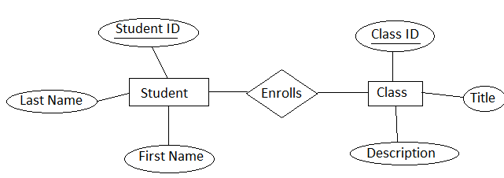
\includegraphics[scale=0.7]{ER_diagram.png}
    \end{center}

    \subsection*{ER-to-Relational Mapping}

    After designing the ER diagram of a system, it needs to be converted to a relational 
    model - so it can be implemented.

    Mapping entities:
    \begin{itemize}
        \item Create a table for each entity
        \item Entity's attributes should become fields of the table with a data type 
        \item Declare primary key (unique identifies)
    \end{itemize}

    Mapping Relationships:
    \begin{itemize}
        \item Create a table for relationships 
        \item Add the primary keys of all participating entities as a field of the table 
        with their data types 
        \item If a relationship has any attributes, add each attribute as a field of the 
        table
        \item Declare a primary key composing all the primary keys of participating 
        entities 
        \item Declare all foreign key constraints
    \end{itemize}

    \begin{center}
        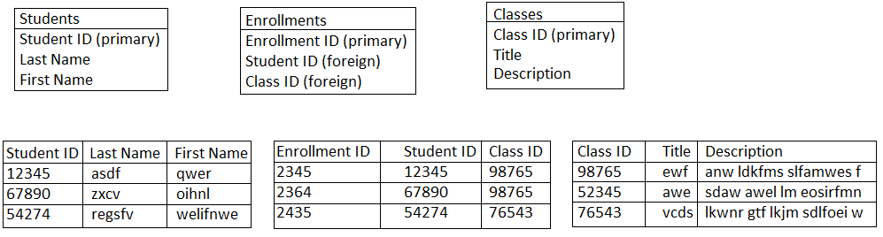
\includegraphics[scale=0.5]{relational_model.png}
    \end{center}

    \subsection*{Intro to SQL}

    Structure Query language - for relational databases. Consists of many types of
    statements - sometimes called sub-languages (data definition DDL and data 
    manipulation DML).

    Data definition language 
    \begin{itemize}
        \item CREATE - creates new databases, tables, and view 
        \item DROP - drops views, tables, and databases 
        \item ALTER - modifies database schema
    \end{itemize}

    Data manipulation language
    \begin{itemize}
        \item SELECT - retrieve a row from a table 
        \item INSERT - add one or more rows to a table 
        \item UPDATE - modifies data of one or more rows from a table 
        \item DELETE - remove one or more rows from a table
    \end{itemize}

    \section*{Software Testing}

    Purpose is to show that a program does what it is intended to do. Executed using 
    artificial data. Can reveal the presence of errors not their absence.

    Devs understand the system but will test "gently" and is driven by delivery. On the 
    other hand, Independent tests must learn about the system but will attempt to break it 
    and is driven by quality.

    \subsection*{Development testing}

    Testing activities carried out by the team developing the system.

    Three stages:
    \begin{itemize}
        \item Unit testing - individual program unites tested. Focuses on functionality of 
        objects or methods 
        \item Component testing - several individual units are integrated to create 
        components. focuses on component interfaces that provide access to the component 
        functions
        \item System testing - some or all of the component are integrated and tested as 
        a whole. focuses on component interactions.
    \end{itemize}

    \subsubsection*{Unit test: black-box testing}

    Know there is specifies function that a product has been design to perform - doesn't 
    know how the system works. Test demonstrate each function is fully operational 
    while searching for errors in each function. Often performed in later stages of testing.

    Example errors:
    \begin{itemize}
        \item incorrect or missing functions 
        \item interface errors 
        \item errors in data structures or external database access 
        \item performance errors 
        \item initialization and termination errors 
    \end{itemize}

    \subsubsection*{White-box testing}

    Knows the internal workings of a product. test ensure that internal operations are 
    performed according to specifications. Selective testing.

    Control-flow-based testing. 1) from the source create a graph describing the flow of 
    control. 2) design test cases to cover certain elements of this graph 
    
    \begin{center}
        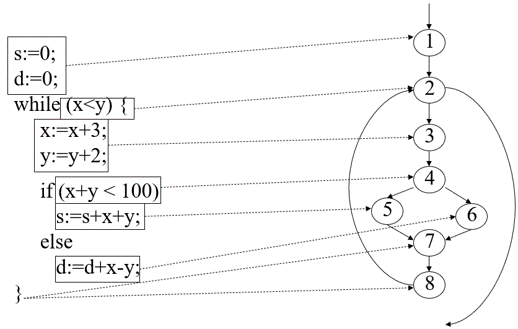
\includegraphics[scale=0.6]{control-flow-graph.png}
    \end{center}

    \subsubsection*{Code coverage}

    Metric used to verify how much of the code has been tested.
    
    \begin{itemize}
        \item Statement coverage - every statement in the code is executed at least once 
        \item Branch coverage - every possible branch from a decision node is 
        executed at least once. considered a necessary testing minimum
        \item Condition coverage - each boolean expression has been tested with a true 
        false value
    \end{itemize}

    \subsubsection*{Partition testing}

    Input data and output results falls into different classes. each of these classes belong
    to an equivalent partition or domain. test cases should be chosen from each partition.

    \begin{center}
        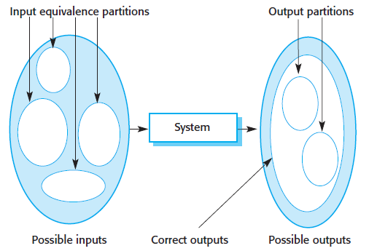
\includegraphics[scale=0.7]{partition-testing.png}
        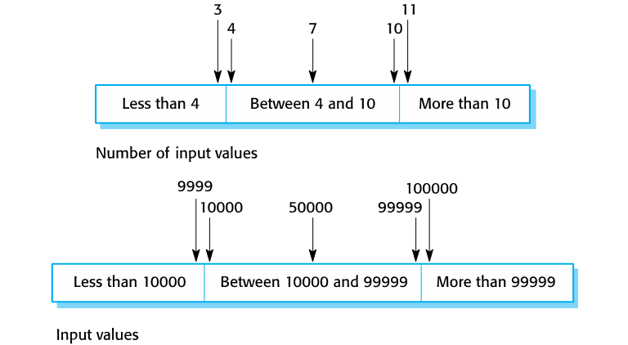
\includegraphics[scale=0.6]{equivalence-partitions.png}
    \end{center}

    \subsubsection*{Boundary value analysis (BVA)}

    Complements equivalence partitioning. test cases on the boundary and midpoint of a 
    partition.

    Guidelines:
    \begin{itemize}
        \item if input condition range is bounded by a and b, then test cases should 
        include a, a-1, a+1, b, b-1, b+1
        \item if input condition specifies a number of values, test cases should include 
        min and max values, as well as values just above and below min/max
        \item If internal data structures have prescribed boundaries, test boundaries 
        (almost full, full, overflow)
    \end{itemize}

    \subsubsection*{General testing guidelines}

    \begin{itemize}
        \item Choose inputs that force the system to generate all error messages
        \item Design inputs that cause buffers to overflow
        \item Repeat the same input or series of inputs numerous times 
        \item Force invalid outputs to be generated
    \end{itemize}

    \subsection*{Component Testing}

    Test cases are not applied to an individual component but to the interface of the 
    composite component created by combining components 

    \begin{itemize}
        \item parameter interfaces - data or function references are passed from one 
        component to another 
        \item shared memory interfaces - a block of memory is shared between components.
        data placed in memory by one component can be accessed by a different one. 
        \item procedural interfaces - one component encapsulates a set of procedures 
        that can be called by other components 
        \item message passing interfaces - one component passes a message to request a 
        service from another component. a return message includes results of 
        executing that service.
    \end{itemize}

    Helps find three main types of errors:
    \begin{itemize}
        \item interface misuse - component calls another component and makes an error in 
        use of its interface (parameters are the wrong type, passed in wrong order etc.)
        \item interface misunderstanding - misunderstand the specification to call a 
        component and make an incorrect assumption about its behavior (binary search 
        is called with an unordered array, making the search fail etc.)
        \item Time errors - occurs in real-time systems that use shared memory or 
        message passing interface (out of date information etc.)
    \end{itemize}

    Guidelines:
    \begin{itemize}
        \item Examine code and identify each call to an external component 
        \item Where pointers are passed, always test interfaces with null pointer parameters
        \item Where a component is called through a procedural interface, design tests to 
        deliberately cause the component to fail
        \item perform stress testing on message passing systems 
        \item where several components interact through shared memory, design tests to vary
        the order the components are activated.
    \end{itemize}

    \subsection*{System testing}

    testing an integrated system. checks that components are compatible, interact 
    correctly, and transfer the right data at the right time. Overlaps with component testing 

    differences:
    \begin{itemize}
        \item Reusable components may have been developed separately. Component testing
        usually looks that the components currently being developed.
        \item components developed by different teams may be integrated. Sometimes 
        system testing is performed by a team with no involvement w/ designers and devs.
    \end{itemize}

    Use-case testing is often used. Sequence diagrams are helpful.

\end{document}